\begin {tikzpicture}[-latex ,auto ,node distance =4 cm and 5cm ,on grid ,
semithick ,
state/.style ={ circle ,top color =white , bottom color = processblue!20 ,
draw,processblue , text=blue , minimum width =1 cm}]
\node[state] (C) {$1$};
\node[state] (A) [above left=of C] {$0$};
\node[state] (B) [above right =of C] {$2$};
\path (A) edge [loop left] node[left] {$1/4$} (A);
\path (C) edge [bend left =25] node[below =0.15 cm] {$1/2$} (A);
\path (A) edge [bend right = -15] node[below =0.15 cm] {$1/2$} (C);
\path (A) edge [bend left =25] node[above] {$1/4$} (B);
\path (B) edge [bend left =15] node[below =0.15 cm] {$1/2$} (A);
\path (C) edge [bend left =15] node[below =0.15 cm] {$1/2$} (B);
\path (B) edge [bend right = -25] node[below =0.15 cm] {$1/2$} (C);
\end{tikzpicture}

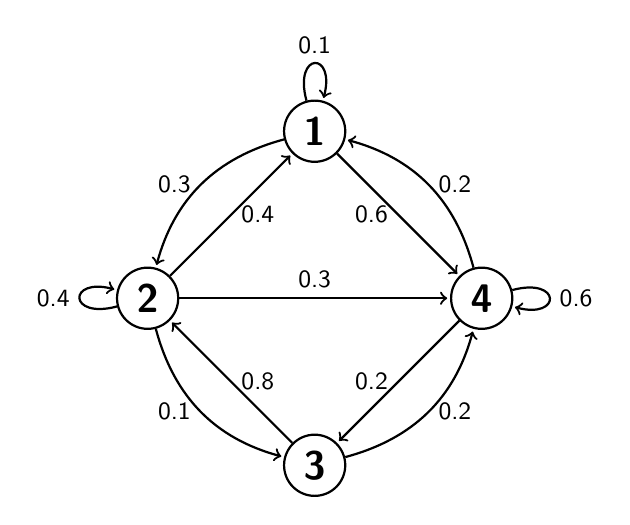
\begin{tikzpicture}[->,shorten >=1pt,auto,node distance=3cm,
                    thick,main node/.style={circle,draw,font=\sffamily\Large\bfseries}]

  \node[main node] (1) {1};
  \node[main node] (2) [below left of=1] {2};
  \node[main node] (3) [below right of=2] {3};
  \node[main node] (4) [below right of=1] {4};

  \path[every node/.style={font=\sffamily\small}]
    (1) edge node [left] {0.6} (4)
        edge [bend right] node[left] {0.3} (2)
        edge [loop above] node {0.1} (1)
    (2) edge node [right] {0.4} (1)
        edge node {0.3} (4)
        edge [loop left] node {0.4} (2)
        edge [bend right] node[left] {0.1} (3)
    (3) edge node [right] {0.8} (2)
        edge [bend right] node[right] {0.2} (4)
    (4) edge node [left] {0.2} (3)
        edge [loop right] node {0.6} (4)
        edge [bend right] node[right] {0.2} (1);
\end{tikzpicture}
